\documentclass[twoside]{book}

% Packages required by doxygen
\usepackage{fixltx2e}
\usepackage{calc}
\usepackage{doxygen}
\usepackage[export]{adjustbox} % also loads graphicx
\usepackage{graphicx}
\usepackage[utf8]{inputenc}
\usepackage{makeidx}
\usepackage{multicol}
\usepackage{multirow}
\PassOptionsToPackage{warn}{textcomp}
\usepackage{textcomp}
\usepackage[nointegrals]{wasysym}
\usepackage[table]{xcolor}

% Font selection
\usepackage[T1]{fontenc}
\usepackage[scaled=.90]{helvet}
\usepackage{courier}
\usepackage{amssymb}
\usepackage{sectsty}
\renewcommand{\familydefault}{\sfdefault}
\allsectionsfont{%
  \fontseries{bc}\selectfont%
  \color{darkgray}%
}
\renewcommand{\DoxyLabelFont}{%
  \fontseries{bc}\selectfont%
  \color{darkgray}%
}
\newcommand{\+}{\discretionary{\mbox{\scriptsize$\hookleftarrow$}}{}{}}

% Page & text layout
\usepackage{geometry}
\geometry{%
  a4paper,%
  top=2.5cm,%
  bottom=2.5cm,%
  left=2.5cm,%
  right=2.5cm%
}
\tolerance=750
\hfuzz=15pt
\hbadness=750
\setlength{\emergencystretch}{15pt}
\setlength{\parindent}{0cm}
\setlength{\parskip}{3ex plus 2ex minus 2ex}
\makeatletter
\renewcommand{\paragraph}{%
  \@startsection{paragraph}{4}{0ex}{-1.0ex}{1.0ex}{%
    \normalfont\normalsize\bfseries\SS@parafont%
  }%
}
\renewcommand{\subparagraph}{%
  \@startsection{subparagraph}{5}{0ex}{-1.0ex}{1.0ex}{%
    \normalfont\normalsize\bfseries\SS@subparafont%
  }%
}
\makeatother

% Headers & footers
\usepackage{fancyhdr}
\pagestyle{fancyplain}
\fancyhead[LE]{\fancyplain{}{\bfseries\thepage}}
\fancyhead[CE]{\fancyplain{}{}}
\fancyhead[RE]{\fancyplain{}{\bfseries\leftmark}}
\fancyhead[LO]{\fancyplain{}{\bfseries\rightmark}}
\fancyhead[CO]{\fancyplain{}{}}
\fancyhead[RO]{\fancyplain{}{\bfseries\thepage}}
\fancyfoot[LE]{\fancyplain{}{}}
\fancyfoot[CE]{\fancyplain{}{}}
\fancyfoot[RE]{\fancyplain{}{\bfseries\scriptsize Generated by Doxygen }}
\fancyfoot[LO]{\fancyplain{}{\bfseries\scriptsize Generated by Doxygen }}
\fancyfoot[CO]{\fancyplain{}{}}
\fancyfoot[RO]{\fancyplain{}{}}
\renewcommand{\footrulewidth}{0.4pt}
\renewcommand{\chaptermark}[1]{%
  \markboth{#1}{}%
}
\renewcommand{\sectionmark}[1]{%
  \markright{\thesection\ #1}%
}

% Indices & bibliography
\usepackage{natbib}
\usepackage[titles]{tocloft}
\setcounter{tocdepth}{3}
\setcounter{secnumdepth}{5}
\makeindex

% Custom commands
\newcommand{\clearemptydoublepage}{%
  \newpage{\pagestyle{empty}\cleardoublepage}%
}

\usepackage{caption}
\captionsetup{labelsep=space,justification=centering,font={bf},singlelinecheck=off,skip=4pt,position=top}

%===== C O N T E N T S =====

\begin{document}

% Titlepage & ToC
\pagenumbering{roman}
\begin{titlepage}
\vspace*{7cm}
\begin{center}%
{\Large Entrées et Sorties Bufferisées }\\
\vspace*{1cm}
{\large Generated by Doxygen 1.8.11}\\
\end{center}
\end{titlepage}
\clearemptydoublepage
\tableofcontents
\clearemptydoublepage
\pagenumbering{arabic}

%--- Begin generated contents ---
\chapter{Lectures et Écriture bufferisées}
\label{md_README}
Barona Stephanie, Grand Maxence

\subsection*{Compilation}


\begin{DoxyCode}
1 make all
\end{DoxyCode}


\subsection*{Exécution}

\subsubsection*{main}

Ce programme lit un fichier donné en argument, et écrit le contenu lu dans un autre fichier. Ce programme est compilé normalement.


\begin{DoxyCode}
1 ./main <filename1> <filename2>
\end{DoxyCode}

\begin{DoxyItemize}
\item filename1 \+: Le fichier à lire
\item filename2 \+: Le fichier à écrire
\end{DoxyItemize}

\subsubsection*{main\+\_\+static}

Ce programme lit un fichier donné en argument, et écrit le contenu lu dans un autre fichier. Ce programme est compilé avec une bibliothèque statique.


\begin{DoxyCode}
1 ./main\_static <filename1> <filename2>
\end{DoxyCode}

\begin{DoxyItemize}
\item filename1 \+: Le fichier à lire
\item filename2 \+: Le fichier à écrire
\end{DoxyItemize}

\subsubsection*{main\+\_\+dyn}

Ce programme lit un fichier donné en argument, et écrit le contenu lu dans un autre fichier. Ce programme est compilé avec une bibliothèque dynamique.


\begin{DoxyCode}
1 ./main\_dyn <filename1> <filename2>
\end{DoxyCode}

\begin{DoxyItemize}
\item filename1 \+: Le fichier à lire
\item filename2 \+: Le fichier à écrire
\end{DoxyItemize}

\subsubsection*{generator}

Ce programme écrit un fichier au contenu et à la taille aléatoire dans un fichier.


\begin{DoxyCode}
1 ./generator <filename>
\end{DoxyCode}

\begin{DoxyItemize}
\item filename \+: Le fichier cible
\end{DoxyItemize}

\subsubsection*{test\+\_\+format}

Ce programme écrit une chaîne formatée dans un fichier, puis la relis et verifie que les valeurs lues sont toujours les mêmes.


\begin{DoxyCode}
1 ./test\_format <filename1>
\end{DoxyCode}

\begin{DoxyItemize}
\item filename1 \+: Le fichier où sera écrite puis lue la chaîne formatée
\end{DoxyItemize}

\subsection*{Tests}


\begin{DoxyCode}
1 make tests
\end{DoxyCode}


Le tests sont effectuées par le script script\+\_\+test.\+sh \+:
\begin{DoxyItemize}
\item Test les fonctions d\textquotesingle{}écritures et lectures bufférisées avec le programme test\+\_\+format
\item Génère des fichiers au contenu et à la taille aléatoire, donne ce fichier en entré du programme main (resp main\+\_\+static main\+\_\+dyn) et vérifie que le fichier $<$filename2$>$ est identique au fichier $<$filename1$>$ 
\end{DoxyItemize}
\chapter{Data Structure Index}
\section{Data Structures}
Here are the data structures with brief descriptions\+:\begin{DoxyCompactList}
\item\contentsline{section}{\hyperlink{structbfile}{bfile} }{\pageref{structbfile}}{}
\end{DoxyCompactList}

\chapter{File Index}
\section{File List}
Here is a list of all documented files with brief descriptions\+:\begin{DoxyCompactList}
\item\contentsline{section}{\hyperlink{bfile_8c}{bfile.\+c} }{\pageref{bfile_8c}}{}
\item\contentsline{section}{\hyperlink{format__in__out_8c}{format\+\_\+in\+\_\+out.\+c} \\*Implémentation des écritures et lectures formatées }{\pageref{format__in__out_8c}}{}
\item\contentsline{section}{include/{\bfseries bfile.\+h} }{\pageref{bfile_8h}}{}
\item\contentsline{section}{include/{\bfseries format\+\_\+in\+\_\+out.\+h} }{\pageref{format__in__out_8h}}{}
\end{DoxyCompactList}

\chapter{Data Structure Documentation}
\hypertarget{structbfile}{}\section{bfile Struct Reference}
\label{structbfile}\index{bfile@{bfile}}
\subsection*{Data Fields}
\begin{DoxyCompactItemize}
\item 
F\+I\+LE $\ast$ {\bfseries f}\hypertarget{structbfile_a3efb0e1a16208deecbd84c15401f7cf8}{}\label{structbfile_a3efb0e1a16208deecbd84c15401f7cf8}

\item 
char {\bfseries mode}\hypertarget{structbfile_a000e34997df38c2005a83d63e67d9282}{}\label{structbfile_a000e34997df38c2005a83d63e67d9282}

\item 
char $\ast$ {\bfseries buffer}\hypertarget{structbfile_aff2566f4c366b48d73479bef43ee4d2e}{}\label{structbfile_aff2566f4c366b48d73479bef43ee4d2e}

\item 
unsigned {\bfseries file\+\_\+seek}\hypertarget{structbfile_a3b0be3218e5b929399c4d9e7679f09a8}{}\label{structbfile_a3b0be3218e5b929399c4d9e7679f09a8}

\item 
unsigned {\bfseries buffer\+\_\+seek}\hypertarget{structbfile_aca30292a051fc4985314320d3cbf9fa4}{}\label{structbfile_aca30292a051fc4985314320d3cbf9fa4}

\item 
size\+\_\+t {\bfseries size\+\_\+buffer}\hypertarget{structbfile_abef66a7af40c1b491eceb9cda4e788a2}{}\label{structbfile_abef66a7af40c1b491eceb9cda4e788a2}

\item 
unsigned {\bfseries eof}\hypertarget{structbfile_aef4112a8c58f34b92863e0fe240d791f}{}\label{structbfile_aef4112a8c58f34b92863e0fe240d791f}

\end{DoxyCompactItemize}


\subsection{Detailed Description}
pour les écritures et lectures bufferisées


\begin{DoxyParams}{Parameters}
{\em f} & \+: le fichier \\
\hline
{\em mode} & \+: Mode de lecteur, E pour écriture, L pour lecture \\
\hline
{\em buffer} & \+: Notre tampon \\
\hline
{\em file\+\_\+seek} & \+: Curseur de f \\
\hline
{\em file\+\_\+seek} & \+: Curseur de buffer \\
\hline
{\em size\+\_\+buffer} & \+: taille du buffer \\
\hline
{\em eof} & \+: booléen indiquant si il reste des choses `a lire dans le fichier \\
\hline
\end{DoxyParams}


The documentation for this struct was generated from the following file\+:\begin{DoxyCompactItemize}
\item 
\hyperlink{bfile_8c}{bfile.\+c}\end{DoxyCompactItemize}

\chapter{File Documentation}
\section{bfile.\+c File Reference}
\label{bfile_8c}\index{bfile.\+c@{bfile.\+c}}


Implémentation des écritures et lectures bufférisées.  


{\ttfamily \#include \char`\"{}include/format\+\_\+in\+\_\+out.\+h\char`\"{}}\\*
{\ttfamily \#include \char`\"{}include/bfile.\+h\char`\"{}}\\*
{\ttfamily \#include $<$stdio.\+h$>$}\\*
{\ttfamily \#include $<$stdlib.\+h$>$}\\*
{\ttfamily \#include $<$stdarg.\+h$>$}\\*
{\ttfamily \#include $<$sys/types.\+h$>$}\\*
Include dependency graph for bfile.\+c\+:
\nopagebreak
\begin{figure}[H]
\begin{center}
\leavevmode
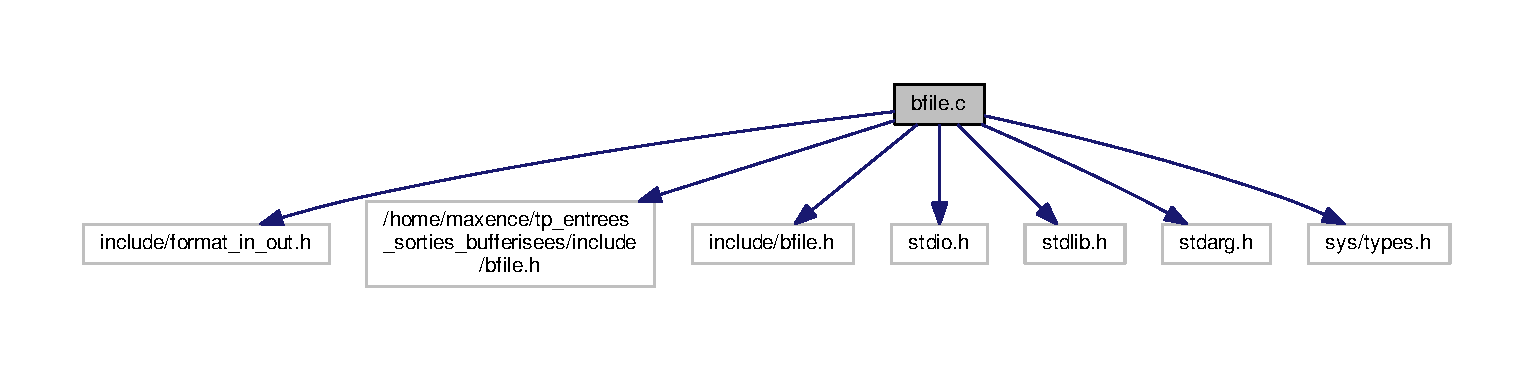
\includegraphics[width=350pt]{bfile_8c__incl}
\end{center}
\end{figure}
\subsection*{Data Structures}
\begin{DoxyCompactItemize}
\item 
struct {\bf bfile}
\begin{DoxyCompactList}\small\item\em Structure pour les écritures et lectures bufferisées. \end{DoxyCompactList}\end{DoxyCompactItemize}
\subsection*{Functions}
\begin{DoxyCompactItemize}
\item 
{\bf bfile} $\ast$ {\bf b\+Open} (const char $\ast$path, char mode)
\begin{DoxyCompactList}\small\item\em Le but de la fonction est d\textquotesingle{}ouvrir le fichier path avec le mode d\textquotesingle{}ouverture en lecture \textquotesingle{}L\textquotesingle{} ou en écriture \textquotesingle{}E\textquotesingle{} et d\textquotesingle{}allouer la structure de bfile avec son tampon et son fichier. La fonction renvoie N\+U\+LL si le fichier ne peut pas être ouvert, un bfile sinon. \end{DoxyCompactList}\item 
int {\bf b\+Close} ({\bf bfile} $\ast$bf)
\begin{DoxyCompactList}\small\item\em Le but de la fonction est de fermer et libérée le fichier pointé sur la structure de donnée de type bfile. \end{DoxyCompactList}\item 
int {\bf b\+Write} (void $\ast$p, int size, int nb\+\_\+element, {\bf bfile} $\ast$bf)
\begin{DoxyCompactList}\small\item\em Le but de la fonction est d\textquotesingle{}écrire nb\+\_\+element de size octets stockés à l’emplacement mémoire pointé par p, dans le tampon. \end{DoxyCompactList}\item 
int {\bf b\+Read} (void $\ast$p, int size, int nb\+\_\+element, {\bf bfile} $\ast$bf)
\begin{DoxyCompactList}\small\item\em Le but de la fonction est de lire nb\+\_\+element de size octets dans bf et y stocker à l’emplacement mémoire pointé par p/. \end{DoxyCompactList}\item 
int {\bf b\+Flush} ({\bf bfile} $\ast$bf)
\begin{DoxyCompactList}\small\item\em Le but de la fonction est xde vider le tampon dans le fichier f. \end{DoxyCompactList}\item 
int {\bf b\+Fill} ({\bf bfile} $\ast$bf)
\begin{DoxyCompactList}\small\item\em Le but de la fonction est de remplir le tampon avec le fichier f. \end{DoxyCompactList}\end{DoxyCompactItemize}


\subsection{Detailed Description}
Implémentation des écritures et lectures bufférisées. 



\subsection{Function Documentation}
\index{bfile.\+c@{bfile.\+c}!b\+Close@{b\+Close}}
\index{b\+Close@{b\+Close}!bfile.\+c@{bfile.\+c}}
\subsubsection[{b\+Close(bfile $\ast$bf)}]{\setlength{\rightskip}{0pt plus 5cm}int b\+Close (
\begin{DoxyParamCaption}
\item[{{\bf bfile} $\ast$}]{bf}
\end{DoxyParamCaption}
)}\label{bfile_8c_a8e8ade7f5d2f2a5d15d1f55e29ebe37c}


Le but de la fonction est de fermer et libérée le fichier pointé sur la structure de donnée de type bfile. 


\begin{DoxyParams}{Parameters}
{\em bf} & \+: la structure à fermer\\
\hline
\end{DoxyParams}
\begin{DoxyReturn}{Returns}
Un entier retourné par la fonction fclose 
\end{DoxyReturn}
\index{bfile.\+c@{bfile.\+c}!b\+Fill@{b\+Fill}}
\index{b\+Fill@{b\+Fill}!bfile.\+c@{bfile.\+c}}
\subsubsection[{b\+Fill(bfile $\ast$bf)}]{\setlength{\rightskip}{0pt plus 5cm}int b\+Fill (
\begin{DoxyParamCaption}
\item[{{\bf bfile} $\ast$}]{bf}
\end{DoxyParamCaption}
)}\label{bfile_8c_ad9ef0d4831a1c1b5b59fdc7e6028c304}


Le but de la fonction est de remplir le tampon avec le fichier f. 


\begin{DoxyParams}{Parameters}
{\em bf} & \\
\hline
\end{DoxyParams}
\begin{DoxyReturn}{Returns}
Le nombre d\textquotesingle{}octet lu dans le fichier 
\end{DoxyReturn}
\index{bfile.\+c@{bfile.\+c}!b\+Flush@{b\+Flush}}
\index{b\+Flush@{b\+Flush}!bfile.\+c@{bfile.\+c}}
\subsubsection[{b\+Flush(bfile $\ast$bf)}]{\setlength{\rightskip}{0pt plus 5cm}int b\+Flush (
\begin{DoxyParamCaption}
\item[{{\bf bfile} $\ast$}]{bf}
\end{DoxyParamCaption}
)}\label{bfile_8c_a7b4b368e4c7ce8305cff87f5461cbca2}


Le but de la fonction est xde vider le tampon dans le fichier f. 


\begin{DoxyParams}{Parameters}
{\em bf} & \\
\hline
\end{DoxyParams}
\begin{DoxyReturn}{Returns}
Le nombre d\textquotesingle{}octet écrit dans le fichier 
\end{DoxyReturn}
\index{bfile.\+c@{bfile.\+c}!b\+Open@{b\+Open}}
\index{b\+Open@{b\+Open}!bfile.\+c@{bfile.\+c}}
\subsubsection[{b\+Open(const char $\ast$path, char mode)}]{\setlength{\rightskip}{0pt plus 5cm}{\bf bfile} $\ast$ b\+Open (
\begin{DoxyParamCaption}
\item[{const char $\ast$}]{path, }
\item[{char}]{mode}
\end{DoxyParamCaption}
)}\label{bfile_8c_ade9460a260a2d4967ba770011bef83fd}


Le but de la fonction est d\textquotesingle{}ouvrir le fichier path avec le mode d\textquotesingle{}ouverture en lecture \textquotesingle{}L\textquotesingle{} ou en écriture \textquotesingle{}E\textquotesingle{} et d\textquotesingle{}allouer la structure de bfile avec son tampon et son fichier. La fonction renvoie N\+U\+LL si le fichier ne peut pas être ouvert, un bfile sinon. 


\begin{DoxyParams}{Parameters}
{\em path} & \+: le nom du fichier \\
\hline
{\em mode} & \+: le mode d\textquotesingle{}ouverture \\
\hline
\end{DoxyParams}
\begin{DoxyReturn}{Returns}
le bfile créé 
\end{DoxyReturn}
\index{bfile.\+c@{bfile.\+c}!b\+Read@{b\+Read}}
\index{b\+Read@{b\+Read}!bfile.\+c@{bfile.\+c}}
\subsubsection[{b\+Read(void $\ast$p, int size, int nb\+\_\+element, bfile $\ast$bf)}]{\setlength{\rightskip}{0pt plus 5cm}int b\+Read (
\begin{DoxyParamCaption}
\item[{void $\ast$}]{p, }
\item[{int}]{size, }
\item[{int}]{nb\+\_\+element, }
\item[{{\bf bfile} $\ast$}]{bf}
\end{DoxyParamCaption}
)}\label{bfile_8c_a5e4cf066a33f4d82aa991ab71c7053dc}


Le but de la fonction est de lire nb\+\_\+element de size octets dans bf et y stocker à l’emplacement mémoire pointé par p/. 


\begin{DoxyParams}{Parameters}
{\em p} & \+: le pointeur à remplir \\
\hline
{\em size} & \+: la taille des données à lrie \\
\hline
{\em nb\+\_\+element} & \+: le nombre de fois que nous lisons. \\
\hline
{\em bf} & \\
\hline
\end{DoxyParams}
\begin{DoxyReturn}{Returns}
Le nombre d’octets lus. 
\end{DoxyReturn}
\index{bfile.\+c@{bfile.\+c}!b\+Write@{b\+Write}}
\index{b\+Write@{b\+Write}!bfile.\+c@{bfile.\+c}}
\subsubsection[{b\+Write(void $\ast$p, int size, int nb\+\_\+element, bfile $\ast$bf)}]{\setlength{\rightskip}{0pt plus 5cm}int b\+Write (
\begin{DoxyParamCaption}
\item[{void $\ast$}]{p, }
\item[{int}]{size, }
\item[{int}]{nb\+\_\+element, }
\item[{{\bf bfile} $\ast$}]{bf}
\end{DoxyParamCaption}
)}\label{bfile_8c_a6c435b2c42c2018b3aa726717b14dfa5}


Le but de la fonction est d\textquotesingle{}écrire nb\+\_\+element de size octets stockés à l’emplacement mémoire pointé par p, dans le tampon. 


\begin{DoxyParams}{Parameters}
{\em p} & \+: le pointeur à écrire \\
\hline
{\em size} & \+: la taille des données à écrire \\
\hline
{\em nb\+\_\+element} & \+: le nombre de fois où on écrit. \\
\hline
{\em bf} & \\
\hline
\end{DoxyParams}
\begin{DoxyReturn}{Returns}
le nombre d’octets écrits 
\end{DoxyReturn}

\section{format\+\_\+in\+\_\+out.\+c File Reference}
\label{format__in__out_8c}\index{format\+\_\+in\+\_\+out.\+c@{format\+\_\+in\+\_\+out.\+c}}
{\ttfamily \#include \char`\"{}include/format\+\_\+in\+\_\+out.\+h\char`\"{}}\\*
{\ttfamily \#include \char`\"{}include/bfile.\+h\char`\"{}}\\*
{\ttfamily \#include $<$stdio.\+h$>$}\\*
{\ttfamily \#include $<$stdlib.\+h$>$}\\*
{\ttfamily \#include $<$stdarg.\+h$>$}\\*
{\ttfamily \#include $<$sys/types.\+h$>$}\\*
{\ttfamily \#include $<$string.\+h$>$}\\*
Include dependency graph for format\+\_\+in\+\_\+out.\+c\+:
\nopagebreak
\begin{figure}[H]
\begin{center}
\leavevmode
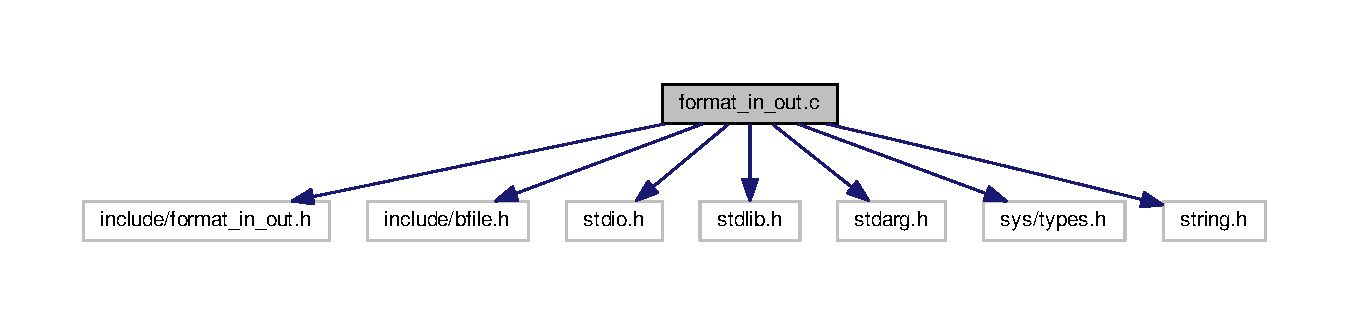
\includegraphics[width=350pt]{format__in__out_8c__incl}
\end{center}
\end{figure}
\subsection*{Functions}
\begin{DoxyCompactItemize}
\item 
char $\ast$ {\bf convert\+\_\+int\+\_\+to\+\_\+str} (int x)
\item 
unsigned {\bf is\+\_\+separator} (char c)
\item 
int {\bf fb\+Write} ({\bf bfile} $\ast$bf, char $\ast$format,...)
\item 
int {\bf fb\+Read} ({\bf bfile} $\ast$bf, char $\ast$format,...)
\end{DoxyCompactItemize}


\subsection{Function Documentation}
\index{format\+\_\+in\+\_\+out.\+c@{format\+\_\+in\+\_\+out.\+c}!convert\+\_\+int\+\_\+to\+\_\+str@{convert\+\_\+int\+\_\+to\+\_\+str}}
\index{convert\+\_\+int\+\_\+to\+\_\+str@{convert\+\_\+int\+\_\+to\+\_\+str}!format\+\_\+in\+\_\+out.\+c@{format\+\_\+in\+\_\+out.\+c}}
\subsubsection[{convert\+\_\+int\+\_\+to\+\_\+str(int x)}]{\setlength{\rightskip}{0pt plus 5cm}char$\ast$ convert\+\_\+int\+\_\+to\+\_\+str (
\begin{DoxyParamCaption}
\item[{int}]{x}
\end{DoxyParamCaption}
)}\label{format__in__out_8c_a0e1b7bbeaceb7e5718f0102f42792c70}
\index{format\+\_\+in\+\_\+out.\+c@{format\+\_\+in\+\_\+out.\+c}!fb\+Read@{fb\+Read}}
\index{fb\+Read@{fb\+Read}!format\+\_\+in\+\_\+out.\+c@{format\+\_\+in\+\_\+out.\+c}}
\subsubsection[{fb\+Read(bfile $\ast$bf, char $\ast$format,...)}]{\setlength{\rightskip}{0pt plus 5cm}int fb\+Read (
\begin{DoxyParamCaption}
\item[{{\bf bfile} $\ast$}]{bf, }
\item[{char $\ast$}]{format, }
\item[{}]{...}
\end{DoxyParamCaption}
)}\label{format__in__out_8c_a58f07ba0af0839a65f606c943bba445e}
\index{format\+\_\+in\+\_\+out.\+c@{format\+\_\+in\+\_\+out.\+c}!fb\+Write@{fb\+Write}}
\index{fb\+Write@{fb\+Write}!format\+\_\+in\+\_\+out.\+c@{format\+\_\+in\+\_\+out.\+c}}
\subsubsection[{fb\+Write(bfile $\ast$bf, char $\ast$format,...)}]{\setlength{\rightskip}{0pt plus 5cm}int fb\+Write (
\begin{DoxyParamCaption}
\item[{{\bf bfile} $\ast$}]{bf, }
\item[{char $\ast$}]{format, }
\item[{}]{...}
\end{DoxyParamCaption}
)}\label{format__in__out_8c_aff97b9e54df890f6a3619d783a13eeaa}
\index{format\+\_\+in\+\_\+out.\+c@{format\+\_\+in\+\_\+out.\+c}!is\+\_\+separator@{is\+\_\+separator}}
\index{is\+\_\+separator@{is\+\_\+separator}!format\+\_\+in\+\_\+out.\+c@{format\+\_\+in\+\_\+out.\+c}}
\subsubsection[{is\+\_\+separator(char c)}]{\setlength{\rightskip}{0pt plus 5cm}unsigned is\+\_\+separator (
\begin{DoxyParamCaption}
\item[{char}]{c}
\end{DoxyParamCaption}
)}\label{format__in__out_8c_a40f14404c0a83290ce9b3eec7e74f98d}

%--- End generated contents ---

% Index
\backmatter
\newpage
\phantomsection
\clearemptydoublepage
\addcontentsline{toc}{chapter}{Index}
\printindex

\end{document}
